\section{Grafos Bipartidos}

\begin{frame}[fragile]{Definição}

    \begin{itemize}
        \item Um grafo é dito bipartido se todos os seus vértices podem ser coloridos usando
            apenas duas cores, de modo que todos os pares de vértices vizinhos tenham cores
            distintas

        \item Tanto a DFS quanto a BFS podem ser utilizadas para verificar se um grafo é 
            bipartido ou não

        \item Inicialmente todos os nós não tem cores atribuídas a eles, e o ponto de partida
            da travessia recebe uma cor (por exemplo, azul)

        \item A travessia continua nos seus vizinhos, que devem receber a cor oposta 
            (por exemplo, vermelho)

        \item Se a travessia atingir um nó já colorido, e a cor dele for a mesma do
            nó que o antecedeu na travessia, o grafo não é bipartido

        \item Uma propriedade interessante dos grafos bipartidos é que eles não podem ter
            ciclos de tamanho ímpar
    \end{itemize}

\end{frame}

\begin{frame}[fragile]{Visualização da identificação de grafos bipartidos}

    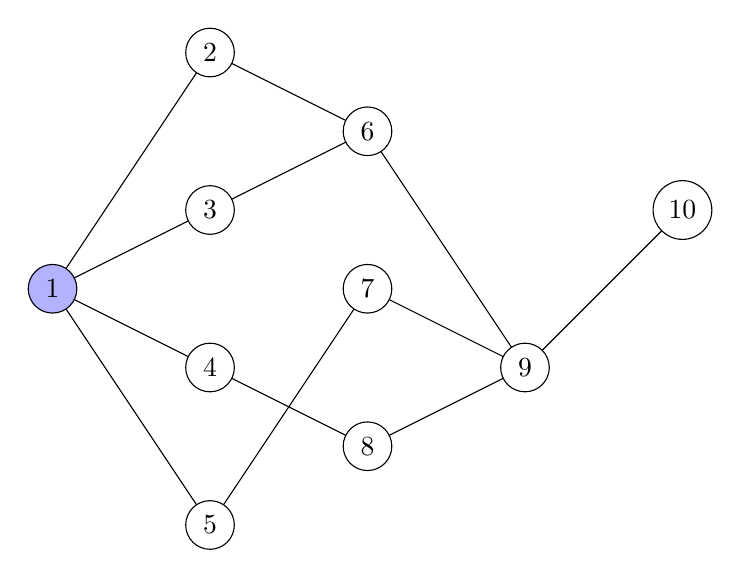
\begin{tikzpicture}
        \draw (0, 5) -- (2, 8);
        \draw (0, 5) -- (2, 6);
        \draw (0, 5) -- (2, 4);
        \draw (0, 5) -- (2, 2);
        \draw (2, 8) -- (4, 7);
        \draw (2, 6) -- (4, 7);
        \draw (2, 4) -- (4, 3);
        \draw (2, 2) -- (4, 5);
        \draw (4, 7) -- (6, 4);
        \draw (4, 5) -- (6, 4);
        \draw (4, 3) -- (6, 4);
        \draw (6, 4) -- (8, 6);

        \node[circle, draw, fill=blue!30] at (0, 5) {1};
        \node[circle, draw, fill=white!30] at (2, 8) {2};
        \node[circle, draw, fill=white!30] at (2, 6) {3};
        \node[circle, draw, fill=white!30] at (2, 4) {4};
        \node[circle, draw, fill=white!30] at (2, 2) {5};
        \node[circle, draw, fill=white!30] at (4, 7) {6};
        \node[circle, draw, fill=white!30] at (4, 5) {7};
        \node[circle, draw, fill=white!30] at (4, 3) {8};
        \node[circle, draw, fill=white!30] at (6, 4) {9};
        \node[circle, draw, fill=white!30] at (8, 6) {10};

    \end{tikzpicture}

\end{frame}

\begin{frame}[fragile]{Visualização da identificação de grafos bipartidos}

    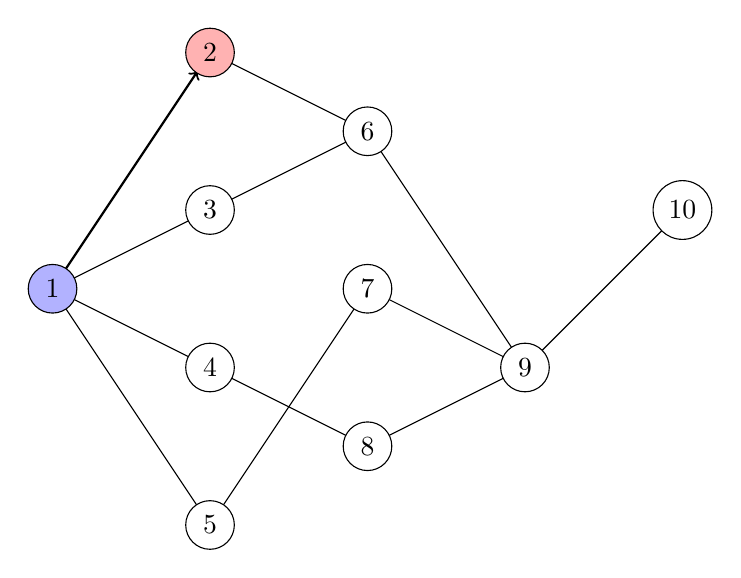
\begin{tikzpicture}
        \draw[thick,->] (0, 5) -- (1.84, 7.76);
        \draw (0, 5) -- (2, 6);
        \draw (0, 5) -- (2, 4);
        \draw (0, 5) -- (2, 2);
        \draw (2, 8) -- (4, 7);
        \draw (2, 6) -- (4, 7);
        \draw (2, 4) -- (4, 3);
        \draw (2, 2) -- (4, 5);
        \draw (4, 7) -- (6, 4);
        \draw (4, 5) -- (6, 4);
        \draw (4, 3) -- (6, 4);
        \draw (6, 4) -- (8, 6);

        \node[circle, draw, fill=blue!30] at (0, 5) {1};
        \node[circle, draw, fill=red!30] at (2, 8) {2};
        \node[circle, draw, fill=white!30] at (2, 6) {3};
        \node[circle, draw, fill=white!30] at (2, 4) {4};
        \node[circle, draw, fill=white!30] at (2, 2) {5};
        \node[circle, draw, fill=white!30] at (4, 7) {6};
        \node[circle, draw, fill=white!30] at (4, 5) {7};
        \node[circle, draw, fill=white!30] at (4, 3) {8};
        \node[circle, draw, fill=white!30] at (6, 4) {9};
        \node[circle, draw, fill=white!30] at (8, 6) {10};

    \end{tikzpicture}

\end{frame}

\begin{frame}[fragile]{Visualização da identificação de grafos bipartidos}

    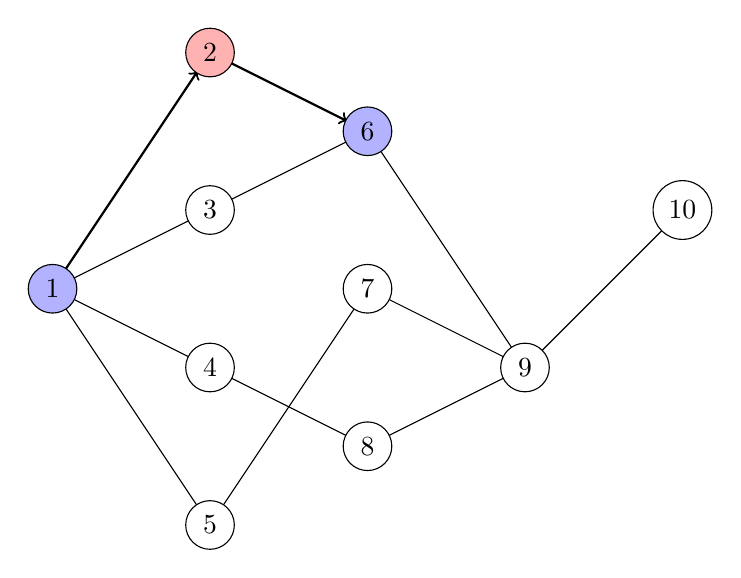
\begin{tikzpicture}
        \draw[thick,->] (0, 5) -- (1.84, 7.76);
        \draw (0, 5) -- (2, 6);
        \draw (0, 5) -- (2, 4);
        \draw (0, 5) -- (2, 2);
        \draw[thick,->] (2, 8) -- (3.74, 7.13);
        \draw (2, 6) -- (4, 7);
        \draw (2, 4) -- (4, 3);
        \draw (2, 2) -- (4, 5);
        \draw (4, 7) -- (6, 4);
        \draw (4, 5) -- (6, 4);
        \draw (4, 3) -- (6, 4);
        \draw (6, 4) -- (8, 6);

        \node[circle, draw, fill=blue!30] at (0, 5) {1};
        \node[circle, draw, fill=red!30] at (2, 8) {2};
        \node[circle, draw, fill=white!30] at (2, 6) {3};
        \node[circle, draw, fill=white!30] at (2, 4) {4};
        \node[circle, draw, fill=white!30] at (2, 2) {5};
        \node[circle, draw, fill=blue!30] at (4, 7) {6};
        \node[circle, draw, fill=white!30] at (4, 5) {7};
        \node[circle, draw, fill=white!30] at (4, 3) {8};
        \node[circle, draw, fill=white!30] at (6, 4) {9};
        \node[circle, draw, fill=white!30] at (8, 6) {10};

    \end{tikzpicture}

\end{frame}

\begin{frame}[fragile]{Visualização da identificação de grafos bipartidos}

    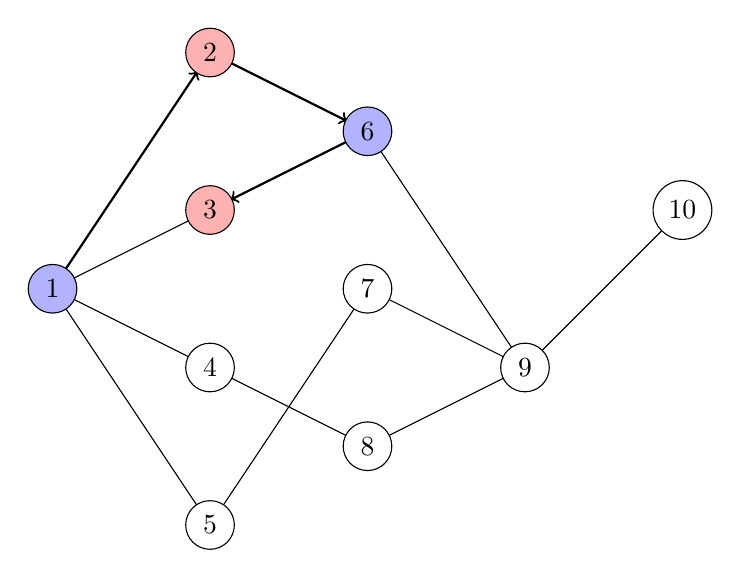
\begin{tikzpicture}
        \draw[thick,->] (0, 5) -- (1.84, 7.76);
        \draw (0, 5) -- (2, 6);
        \draw (0, 5) -- (2, 4);
        \draw (0, 5) -- (2, 2);
        \draw[thick,->] (2, 8) -- (3.74, 7.13);
        \draw[thick,<-] (2.26, 6.13) -- (4, 7);
        \draw (2, 4) -- (4, 3);
        \draw (2, 2) -- (4, 5);
        \draw (4, 7) -- (6, 4);
        \draw (4, 5) -- (6, 4);
        \draw (4, 3) -- (6, 4);
        \draw (6, 4) -- (8, 6);

        \node[circle, draw, fill=blue!30] at (0, 5) {1};
        \node[circle, draw, fill=red!30] at (2, 8) {2};
        \node[circle, draw, fill=red!30] at (2, 6) {3};
        \node[circle, draw, fill=white!30] at (2, 4) {4};
        \node[circle, draw, fill=white!30] at (2, 2) {5};
        \node[circle, draw, fill=blue!30] at (4, 7) {6};
        \node[circle, draw, fill=white!30] at (4, 5) {7};
        \node[circle, draw, fill=white!30] at (4, 3) {8};
        \node[circle, draw, fill=white!30] at (6, 4) {9};
        \node[circle, draw, fill=white!30] at (8, 6) {10};

    \end{tikzpicture}

\end{frame}

\begin{frame}[fragile]{Visualização da identificação de grafos bipartidos}

    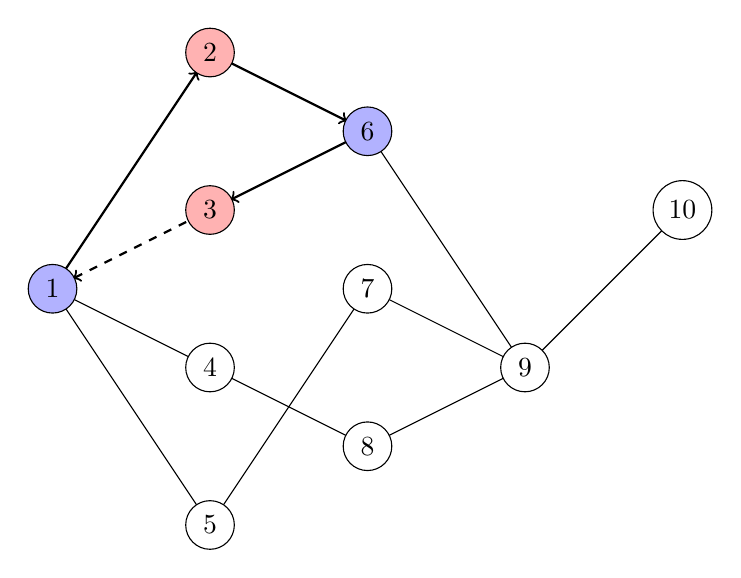
\begin{tikzpicture}
        \draw[thick,->] (0, 5) -- (1.84, 7.76);
        \draw (0, 5) -- (2, 4);
        \draw[thick,<-,dashed] (0.26, 5.13) -- (2, 6);
        \draw (0, 5) -- (2, 2);
        \draw[thick,->] (2, 8) -- (3.74, 7.13);
        \draw[thick,<-] (2.26, 6.13) -- (4, 7);
        \draw (2, 4) -- (4, 3);
        \draw (2, 2) -- (4, 5);
        \draw (4, 7) -- (6, 4);
        \draw (4, 5) -- (6, 4);
        \draw (4, 3) -- (6, 4);
        \draw (6, 4) -- (8, 6);

        \node[circle, draw, fill=blue!30] at (0, 5) {1};
        \node[circle, draw, fill=red!30] at (2, 8) {2};
        \node[circle, draw, fill=red!30] at (2, 6) {3};
        \node[circle, draw, fill=white!30] at (2, 4) {4};
        \node[circle, draw, fill=white!30] at (2, 2) {5};
        \node[circle, draw, fill=blue!30] at (4, 7) {6};
        \node[circle, draw, fill=white!30] at (4, 5) {7};
        \node[circle, draw, fill=white!30] at (4, 3) {8};
        \node[circle, draw, fill=white!30] at (6, 4) {9};
        \node[circle, draw, fill=white!30] at (8, 6) {10};

    \end{tikzpicture}

\end{frame}

\begin{frame}[fragile]{Visualização da identificação de grafos bipartidos}

    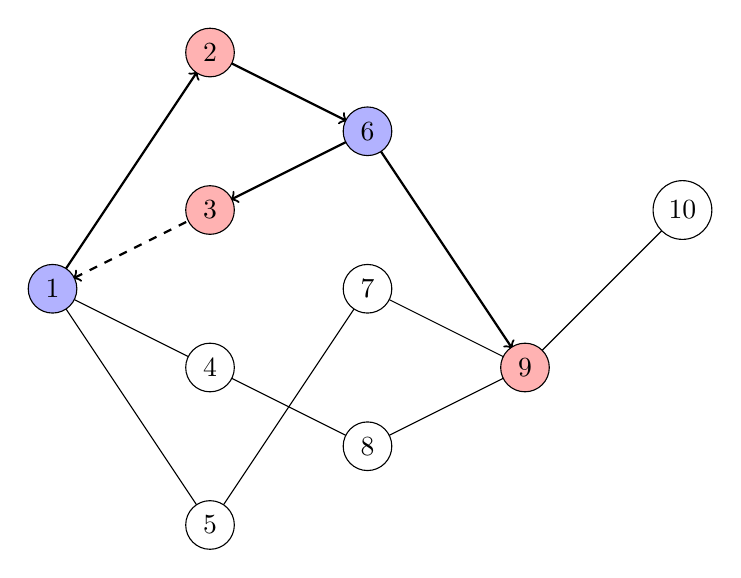
\begin{tikzpicture}
        \draw[thick,->] (0, 5) -- (1.84, 7.76);
        \draw (0, 5) -- (2, 4);
        \draw[thick,<-,dashed] (0.26, 5.13) -- (2, 6);
        \draw (0, 5) -- (2, 2);
        \draw[thick,->] (2, 8) -- (3.74, 7.13);
        \draw[thick,<-] (2.26, 6.13) -- (4, 7);
        \draw (2, 4) -- (4, 3);
        \draw (2, 2) -- (4, 5);
        \draw[thick,->] (4, 7) -- (5.84, 4.24);
        \draw (4, 5) -- (6, 4);
        \draw (4, 3) -- (6, 4);
        \draw (6, 4) -- (8, 6);

        \node[circle, draw, fill=blue!30] at (0, 5) {1};
        \node[circle, draw, fill=red!30] at (2, 8) {2};
        \node[circle, draw, fill=red!30] at (2, 6) {3};
        \node[circle, draw, fill=white!30] at (2, 4) {4};
        \node[circle, draw, fill=white!30] at (2, 2) {5};
        \node[circle, draw, fill=blue!30] at (4, 7) {6};
        \node[circle, draw, fill=white!30] at (4, 5) {7};
        \node[circle, draw, fill=white!30] at (4, 3) {8};
        \node[circle, draw, fill=red!30] at (6, 4) {9};
        \node[circle, draw, fill=white!30] at (8, 6) {10};

    \end{tikzpicture}

\end{frame}

\begin{frame}[fragile]{Visualização da identificação de grafos bipartidos}

    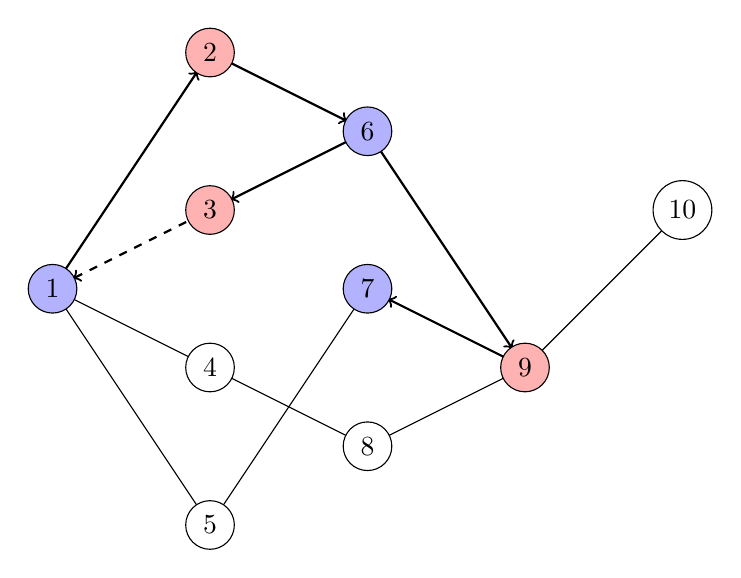
\begin{tikzpicture}
        \draw[thick,->] (0, 5) -- (1.84, 7.76);
        \draw (0, 5) -- (2, 4);
        \draw[thick,<-,dashed] (0.26, 5.13) -- (2, 6);
        \draw (0, 5) -- (2, 2);
        \draw[thick,->] (2, 8) -- (3.74, 7.13);
        \draw[thick,<-] (2.26, 6.13) -- (4, 7);
        \draw (2, 4) -- (4, 3);
        \draw (2, 2) -- (4, 5);
        \draw[thick,->] (4, 7) -- (5.84, 4.24);
        \draw[thick,<-] (4.26, 4.87) -- (6, 4);
        \draw (4, 3) -- (6, 4);
        \draw (6, 4) -- (8, 6);

        \node[circle, draw, fill=blue!30] at (0, 5) {1};
        \node[circle, draw, fill=red!30] at (2, 8) {2};
        \node[circle, draw, fill=red!30] at (2, 6) {3};
        \node[circle, draw, fill=white!30] at (2, 4) {4};
        \node[circle, draw, fill=white!30] at (2, 2) {5};
        \node[circle, draw, fill=blue!30] at (4, 7) {6};
        \node[circle, draw, fill=blue!30] at (4, 5) {7};
        \node[circle, draw, fill=white!30] at (4, 3) {8};
        \node[circle, draw, fill=red!30] at (6, 4) {9};
        \node[circle, draw, fill=white!30] at (8, 6) {10};

    \end{tikzpicture}

\end{frame}

\begin{frame}[fragile]{Visualização da identificação de grafos bipartidos}

    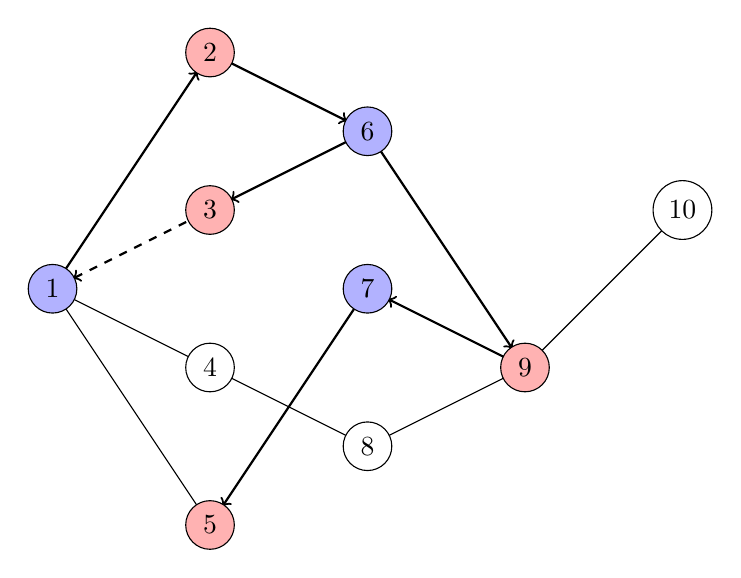
\begin{tikzpicture}
        \draw[thick,->] (0, 5) -- (1.84, 7.76);
        \draw (0, 5) -- (2, 4);
        \draw[thick,<-,dashed] (0.26, 5.13) -- (2, 6);
        \draw (0, 5) -- (2, 2);
        \draw[thick,->] (2, 8) -- (3.74, 7.13);
        \draw[thick,<-] (2.26, 6.13) -- (4, 7);
        \draw (2, 4) -- (4, 3);
        \draw[thick,<-] (2.16, 2.24) -- (4, 5);
        \draw[thick,->] (4, 7) -- (5.84, 4.24);
        \draw[thick,<-] (4.26, 4.87) -- (6, 4);
        \draw (4, 3) -- (6, 4);
        \draw (6, 4) -- (8, 6);

        \node[circle, draw, fill=blue!30] at (0, 5) {1};
        \node[circle, draw, fill=red!30] at (2, 8) {2};
        \node[circle, draw, fill=red!30] at (2, 6) {3};
        \node[circle, draw, fill=white!30] at (2, 4) {4};
        \node[circle, draw, fill=red!30] at (2, 2) {5};
        \node[circle, draw, fill=blue!30] at (4, 7) {6};
        \node[circle, draw, fill=blue!30] at (4, 5) {7};
        \node[circle, draw, fill=white!30] at (4, 3) {8};
        \node[circle, draw, fill=red!30] at (6, 4) {9};
        \node[circle, draw, fill=white!30] at (8, 6) {10};

    \end{tikzpicture}

\end{frame}

\begin{frame}[fragile]{Visualização da identificação de grafos bipartidos}

    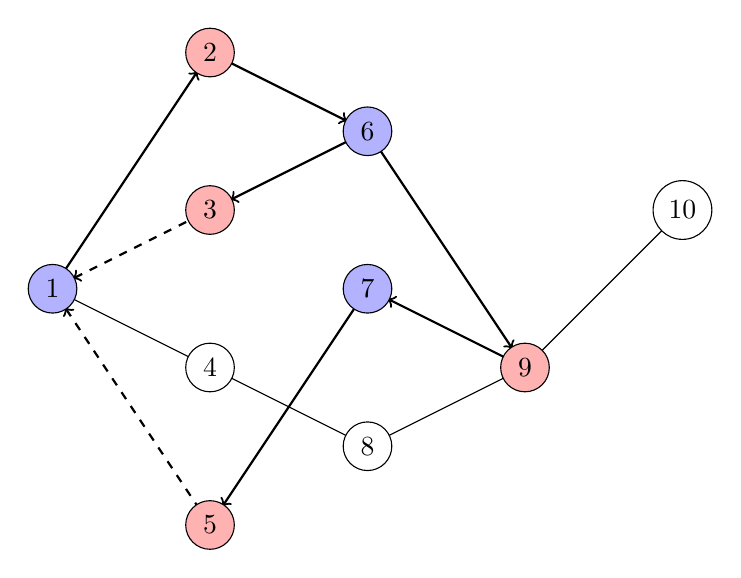
\begin{tikzpicture}
        \draw[thick,->] (0, 5) -- (1.84, 7.76);
        \draw (0, 5) -- (2, 4);
        \draw[thick,<-,dashed] (0.26, 5.13) -- (2, 6);
        \draw[thick,<-,dashed] (0.16, 4.76) -- (2, 2);
        \draw[thick,->] (2, 8) -- (3.74, 7.13);
        \draw[thick,<-] (2.26, 6.13) -- (4, 7);
        \draw (2, 4) -- (4, 3);
        \draw[thick,<-] (2.16, 2.24) -- (4, 5);
        \draw[thick,->] (4, 7) -- (5.84, 4.24);
        \draw[thick,<-] (4.26, 4.87) -- (6, 4);
        \draw (4, 3) -- (6, 4);
        \draw (6, 4) -- (8, 6);

        \node[circle, draw, fill=blue!30] at (0, 5) {1};
        \node[circle, draw, fill=red!30] at (2, 8) {2};
        \node[circle, draw, fill=red!30] at (2, 6) {3};
        \node[circle, draw, fill=white!30] at (2, 4) {4};
        \node[circle, draw, fill=red!30] at (2, 2) {5};
        \node[circle, draw, fill=blue!30] at (4, 7) {6};
        \node[circle, draw, fill=blue!30] at (4, 5) {7};
        \node[circle, draw, fill=white!30] at (4, 3) {8};
        \node[circle, draw, fill=red!30] at (6, 4) {9};
        \node[circle, draw, fill=white!30] at (8, 6) {10};

    \end{tikzpicture}

\end{frame}

\begin{frame}[fragile]{Visualização da identificação de grafos bipartidos}

    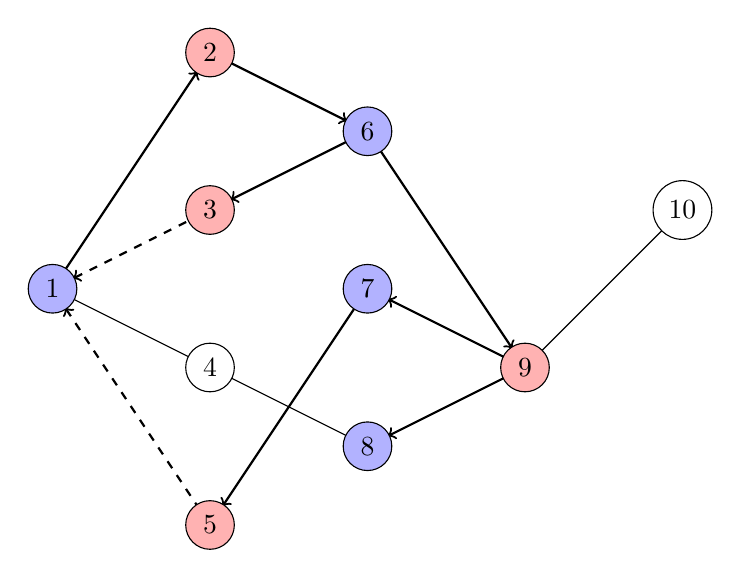
\begin{tikzpicture}
        \draw[thick,->] (0, 5) -- (1.84, 7.76);
        \draw (0, 5) -- (2, 4);
        \draw[thick,<-,dashed] (0.26, 5.13) -- (2, 6);
        \draw[thick,<-,dashed] (0.16, 4.76) -- (2, 2);
        \draw[thick,->] (2, 8) -- (3.74, 7.13);
        \draw[thick,<-] (2.26, 6.13) -- (4, 7);
        \draw (2, 4) -- (4, 3);
        \draw[thick,<-] (2.16, 2.24) -- (4, 5);
        \draw[thick,->] (4, 7) -- (5.84, 4.24);
        \draw[thick,<-] (4.26, 4.87) -- (6, 4);
        \draw[thick,<-] (4.26, 3.13) -- (6, 4);
        \draw (6, 4) -- (8, 6);

        \node[circle, draw, fill=blue!30] at (0, 5) {1};
        \node[circle, draw, fill=red!30] at (2, 8) {2};
        \node[circle, draw, fill=red!30] at (2, 6) {3};
        \node[circle, draw, fill=white!30] at (2, 4) {4};
        \node[circle, draw, fill=red!30] at (2, 2) {5};
        \node[circle, draw, fill=blue!30] at (4, 7) {6};
        \node[circle, draw, fill=blue!30] at (4, 5) {7};
        \node[circle, draw, fill=blue!30] at (4, 3) {8};
        \node[circle, draw, fill=red!30] at (6, 4) {9};
        \node[circle, draw, fill=white!30] at (8, 6) {10};

    \end{tikzpicture}

\end{frame}

\begin{frame}[fragile]{Visualização da identificação de grafos bipartidos}

    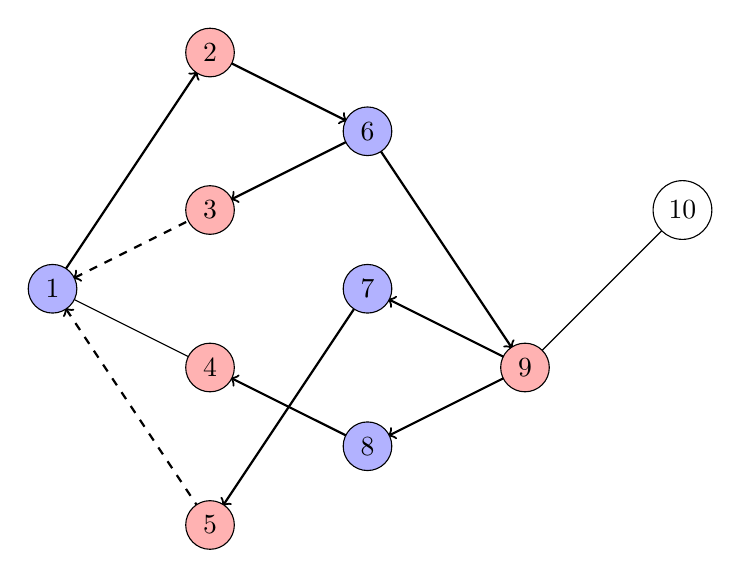
\begin{tikzpicture}
        \draw[thick,->] (0, 5) -- (1.84, 7.76);
        \draw (0, 5) -- (2, 4);
        \draw[thick,<-,dashed] (0.26, 5.13) -- (2, 6);
        \draw[thick,<-,dashed] (0.16, 4.76) -- (2, 2);
        \draw[thick,->] (2, 8) -- (3.74, 7.13);
        \draw[thick,<-] (2.26, 6.13) -- (4, 7);
        \draw[thick,<-] (2.26, 3.87) -- (4, 3);
        \draw[thick,<-] (2.16, 2.24) -- (4, 5);
        \draw[thick,->] (4, 7) -- (5.84, 4.24);
        \draw[thick,<-] (4.26, 4.87) -- (6, 4);
        \draw[thick,<-] (4.26, 3.13) -- (6, 4);
        \draw (6, 4) -- (8, 6);

        \node[circle, draw, fill=blue!30] at (0, 5) {1};
        \node[circle, draw, fill=red!30] at (2, 8) {2};
        \node[circle, draw, fill=red!30] at (2, 6) {3};
        \node[circle, draw, fill=red!30] at (2, 4) {4};
        \node[circle, draw, fill=red!30] at (2, 2) {5};
        \node[circle, draw, fill=blue!30] at (4, 7) {6};
        \node[circle, draw, fill=blue!30] at (4, 5) {7};
        \node[circle, draw, fill=blue!30] at (4, 3) {8};
        \node[circle, draw, fill=red!30] at (6, 4) {9};
        \node[circle, draw, fill=white!30] at (8, 6) {10};

    \end{tikzpicture}

\end{frame}

\begin{frame}[fragile]{Visualização da identificação de grafos bipartidos}

    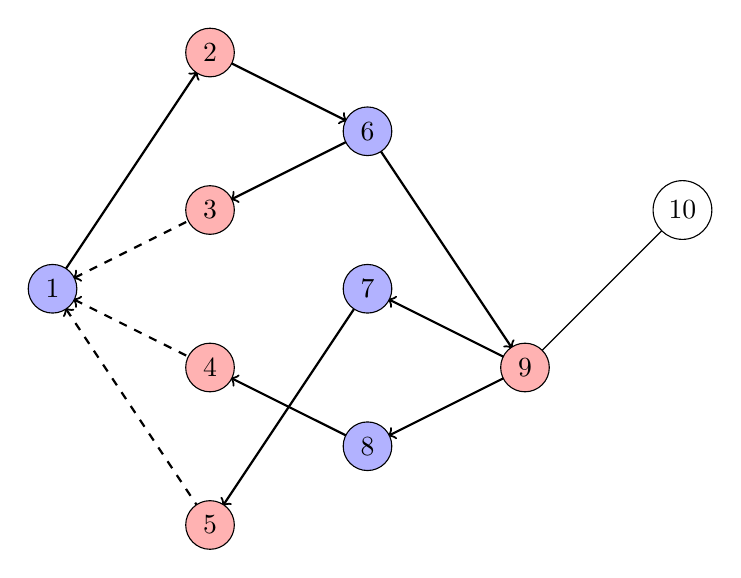
\begin{tikzpicture}
        \draw[thick,->] (0, 5) -- (1.84, 7.76);
        \draw[thick,<-,dashed] (0.26, 4.87) -- (2, 4);
        \draw[thick,<-,dashed] (0.26, 5.13) -- (2, 6);
        \draw[thick,<-,dashed] (0.16, 4.76) -- (2, 2);
        \draw[thick,->] (2, 8) -- (3.74, 7.13);
        \draw[thick,<-] (2.26, 6.13) -- (4, 7);
        \draw[thick,<-] (2.26, 3.87) -- (4, 3);
        \draw[thick,<-] (2.16, 2.24) -- (4, 5);
        \draw[thick,->] (4, 7) -- (5.84, 4.24);
        \draw[thick,<-] (4.26, 4.87) -- (6, 4);
        \draw[thick,<-] (4.26, 3.13) -- (6, 4);
        \draw (6, 4) -- (8, 6);

        \node[circle, draw, fill=blue!30] at (0, 5) {1};
        \node[circle, draw, fill=red!30] at (2, 8) {2};
        \node[circle, draw, fill=red!30] at (2, 6) {3};
        \node[circle, draw, fill=red!30] at (2, 4) {4};
        \node[circle, draw, fill=red!30] at (2, 2) {5};
        \node[circle, draw, fill=blue!30] at (4, 7) {6};
        \node[circle, draw, fill=blue!30] at (4, 5) {7};
        \node[circle, draw, fill=blue!30] at (4, 3) {8};
        \node[circle, draw, fill=red!30] at (6, 4) {9};
        \node[circle, draw, fill=white!30] at (8, 6) {10};

    \end{tikzpicture}

\end{frame}

\begin{frame}[fragile]{Visualização da identificação de grafos bipartidos}

    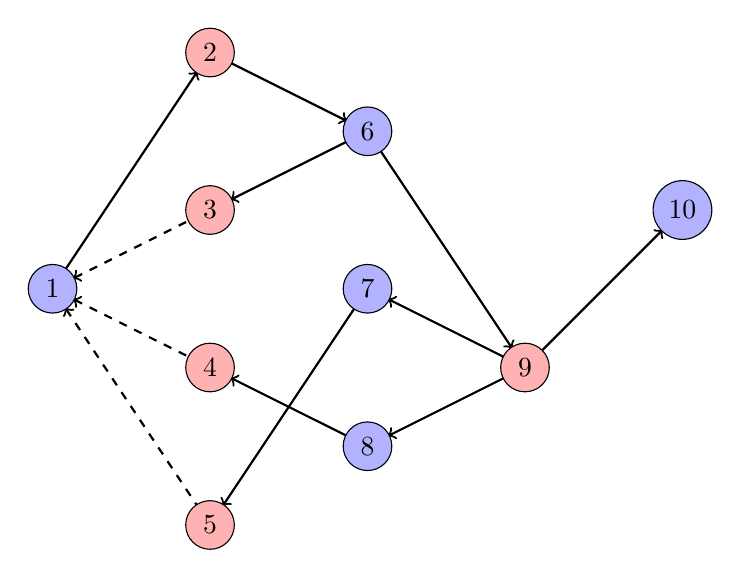
\begin{tikzpicture}
        \draw[thick,->] (0, 5) -- (1.84, 7.76);
        \draw[thick,<-,dashed] (0.26, 4.87) -- (2, 4);
        \draw[thick,<-,dashed] (0.26, 5.13) -- (2, 6);
        \draw[thick,<-,dashed] (0.16, 4.76) -- (2, 2);
        \draw[thick,->] (2, 8) -- (3.74, 7.13);
        \draw[thick,<-] (2.26, 6.13) -- (4, 7);
        \draw[thick,<-] (2.26, 3.87) -- (4, 3);
        \draw[thick,<-] (2.16, 2.24) -- (4, 5);
        \draw[thick,->] (4, 7) -- (5.84, 4.24);
        \draw[thick,<-] (4.26, 4.87) -- (6, 4);
        \draw[thick,<-] (4.26, 3.13) -- (6, 4);
        \draw[thick,->] (6, 4) -- (7.75, 5.75);

        \node[circle, draw, fill=blue!30] at (0, 5) {1};
        \node[circle, draw, fill=red!30] at (2, 8) {2};
        \node[circle, draw, fill=red!30] at (2, 6) {3};
        \node[circle, draw, fill=red!30] at (2, 4) {4};
        \node[circle, draw, fill=red!30] at (2, 2) {5};
        \node[circle, draw, fill=blue!30] at (4, 7) {6};
        \node[circle, draw, fill=blue!30] at (4, 5) {7};
        \node[circle, draw, fill=blue!30] at (4, 3) {8};
        \node[circle, draw, fill=red!30] at (6, 4) {9};
        \node[circle, draw, fill=blue!30] at (8, 6) {10};

    \end{tikzpicture}

\end{frame}

\begin{frame}[fragile]{Implementação da verificação em C++}
    \inputsnippet{c++}{1}{20}{bipartite.cpp}
\end{frame}

\begin{frame}[fragile]{Implementação da verificação em C++}
    \inputsnippet{c++}{21}{41}{bipartite.cpp}
\end{frame}

\begin{frame}[fragile]{Implementação da verificação em C++}
    \inputsnippet{c++}{42}{62}{bipartite.cpp}
\end{frame}
